\chapter{Background}
\label{chapter:background}

In this chapter we introduce the necessary concepts to describe the dynamics of a fully ionized
single species plasma under the influence of many simultaneous particle collisions.
We conclude by presenting the disorder induced heating (\gls{dih}) process and highlight why it is necessary to
model collisions in such a regime.

\section{Notation}

In this section we introduce the notation used throughout the report (it partly follows
the one introduced in \cite{thomas2012review}).
We denote vector quantities with bold font $\vect b$ and tensor quantities with a double underscore $\matr C$.
Individual components of vector or tensor quantities are displayed with subscripts, i.e. $\vect b_i$,
$\matr C_{i,j}$.
Given a normed vector space in $\mathbb R^3$, we can write a rank 2 tensor with orthonormal unit
vectors $\vect e_1, \vect e_2, \vect e_3$, as $\matr C = \sum_{i,j} \matr C_{i,j} \vect e_i \vect e_j$.
A dot between two vectors defines a contraction of the nearest indices $(\nabla \vect b) \cdot \vect d = \sum_j
(\nabla_i \vect b_j) \vect d_j$.
Analogously, a double dot product between tensors is the contraction $\matr C : \matr E = \sum_{i,j}
\matr C_{i,j}
\matr E_{i,j}$.
We define the $L^2$-norm of vectors as $\lVert \vect b \rVert_2 = \sqrt{\sum_i \vert b_i \vert^2}$.
To simplify formulas containing $L^2$-norms of the phase space position and velocity vectors
$(\vect r, \vect v)$, we choose to simplify the notation and use non-bold letters $(r, v)$ instead.

To represent partial differential equations (\gls{pde}s) of vectorial quantities we rely on differential
operators.
We shortly list the operators found in this report.
The operator subscript indicates on what subspace variables it acts on (i.e. $\posNabla$ acts in
configuration space whereas $\velNabla$ acts in velocity space)
\begin{align}
    \begin{split}
    \label{eq:diffGrad}
    \posNabla = \left( \frac{\partial}{\partial \vect r_1}, \frac{\partial}{\partial \vect r_2},
    \frac{\partial}{\partial \vect r_3} \right)^T, %= \text{grad}
    \end{split}
    \eqVspace
    \begin{split}
    \label{eq:diffDiv}
    \Delta_{\vect r} = \posNabla \cdot \posNabla,
    \end{split}
    \eqVspace
    \begin{split}
    \label{eq:diffHess}
    \matr H_{\vect r} = 
        \begin{bmatrix}
            \frac{\partial^2}{\partial \vect r_1 \partial \vect r_1} & \frac{\partial^2}{\partial \vect r_1 \vect r_2} & \frac{\partial^2}{\partial \vect r_1 \vect r_3} \\
            \frac{\partial^2}{\partial \vect r_2 \partial \vect r_1} & \frac{\partial^2}{\partial \vect r_2 \vect r_2} & \frac{\partial^2}{\partial \vect r_2 \vect r_3} \\
            \frac{\partial^2}{\partial \vect r_3 \partial \vect r_1} & \frac{\partial^2}{\partial \vect r_3 \vect r_2} & \frac{\partial^2}{\partial \vect r_3 \vect r_3}
        \end{bmatrix},
    \end{split}
    \eqVspace
    \begin{split}
        \text{Tr}(\matr C) = \sum_i \matr C_{i,i}.
    \end{split}
\end{align}

The method in this report requires a computational mesh as a data structure to store field
quantities.
We define the extents of a field in 3 dimensions as $[0,L_x] \times [0,L_y] \times [0, L_z]$, while the mesh
contains a total of $N_x \times N_y \times N_z$ cells. Thus, the mesh width
or cellwidth along each dimension is $h_x = L_x / N_x,h_y = L_y / N_y, h_z = L_z / N_z$. 
We use a cell centered approach to define the quantities on a mesh: $\vect x_{i,j,k} = (ih_x, jh_y, kh_z)$
with half indices $(i,j,k) \in [\frac{1}{2},\dots,N_x-\frac{1}{2}] \times
[\frac{1}{2},\dots,N_y-\frac{1}{2}] \times [\frac{1}{2},\dots,N_z-\frac{1}{2}]$.
If a field exhibits the same extent along each dimension, we omit the subscript on the mesh
properties ($[0,L]^3$ and $h$).

For mesh quantities in the context of a finite difference (\gls{fd}) scheme, the superscript $\vect x^n = \vect x(t_n)$ defines the state
at timestep $n$. The same quantity at the subsequent timestep is then $\vect x^{n+1} = \vect x(t_n + dt)$.
Similarly, for neighboring mesh cells of $\vect x_{i,j,k}$ we use an index increment (e.g. $\vect
x_{i+1,j,k}$ for its right neighboring cell along the first dimension).

In Tables \ref{table:nomenclature} and \ref{table:plasma_nomenclature} we summarize the nomenclature
we use in this report.

\begin{table}[h]
    \centering
    \caption{Nomenclature used throughout this report.}
    \begin{tabularx}{0.75\textwidth}{l l l}
        \toprule
        Symbol & Definition \\
        \midrule
        $N_{o}$ & Mesh size along one dimension, where $o \in \{x,y,z\}$ \\
        $N_m$ & Total number of cells in a mesh ($N_m = N_x \times N_y \times N_z$) \\
        $N_p$ & Total number of particles \\
        $\eta$ & Relative approximation error $\eta(x, x_{\text{appr}}) = \left(\frac{\lVert x_{\text{appr}}-x \rVert_2}{\lVert x
            \rVert_2} \right)$\\
        \bottomrule
    \end{tabularx}
    \label{table:nomenclature}
\end{table}

\begin{table}[h]
    \centering
    \caption{Nomenclature commonly used in plasma physics.}
    \begin{tabularx}{0.75\textwidth}{l l l}
        \toprule
        Symbol & Definition \\
        \midrule
        $n_0$ & Electron number density\\
        $\lambda_D$ & Debye length \\
        $v_{th}$ & Thermal velocity \\
        $\omega_{p}$ & Plasma frequency \\
        $\tau_{p}$ & Plasma period \\
        $\varepsilon_{0}$ & Vacuum permittivity \\
        $m_e$ & Electron mass \\
        $e$ & Elementary charge \\
        \bottomrule
    \end{tabularx}
    \label{table:plasma_nomenclature}
\end{table}

\section{Coulomb Interactions}
\label{section:coulombInteractions}

The plasma containing charged particles (in our case electrons) can exhibit very 
high density (up to $10^{30}\ \text{m}^{-3}$).
Coulomb's inverse-square law defines the electrostatic force interaction between two particles
located at positions $\vect r_i$ and $\vect r_j$.
The force excerted on particle $i$ by particle $j$ is inversely proportional to the squared distance
$\vect r_{ij} = \vect r_i - \vect r_j$ between the two particles:
\begin{equation}
    \vect F_{ij} = \frac{1}{4 \pi \vp} \frac{q_i q_j}{r_{ij}^2} \hat{\vect r}_{ij},
    \label{eq:coulombForce}
\end{equation}
where $\hat{\vect r}_{ij} = \frac{\vect r_{ij}}{r_{ij}}$ is a unit vector pointing from particle $i$ to
particle $j$. 
These interactions happen collectively, meaning that every particle experiences electric field
forces from neighboring particles while at the same time, they themselves are influenced by particles nearby.

\section{Vlasov-Poisson Equation}
\label{section:vlasov_poisson}

The majority of phenomena arising from particles interacting in a plasma state can be modeled adequately with a
description of fluids (i.e. with Navier-Stokes equation), allowing the analysis of macroscopic
properties such as density and mean energy.
A system that is far away from thermal equilibrium can show a strong dependence on small-scale
structures that need to be properly resolved.
Making use of the velocity distribution of the system can help to better capture these interactions.
Thus, we can express it via a 6d phase space ($\vect r, \vect v$) defined by a
distribution function $f(\vect r, \vect v, t)$, which characterizes the particle density at position
and velocity ($\vect r, \vect v$) at time $t$.

Taking a particle description of a plasma containing $N_p$ particles, we can define its distribution with 
the Dirac delta function:
\begin{equation}
    f_K(\vect r, \vect v, t) = \sum_{i=1}^{N_p} \delta [ \vect r - \vect r_i ] \delta [ \vect v - \vect v_i ].
    \label{eq:klimontovich_distribution}
\end{equation}
This description is also known as the Klimontovich distribution function and grants us the insight
of whether we can expect to find a particle at a certain position $(\vect r, \vect v)$ at time $t$ \cite{nicholson1983}.
But it being zero almost everywhere except at the particle positions $(\vect r, \vect v)$ can be inhibiting
for subsequent computations due to its singular nature.
A better description still, would exhibit at least some smoothness as we are more interested in
averaged quantities.
By integrating over a volume element $dV = \Delta \vect r \Delta \vect v$, containing $N_{dV}(\vect r, \vect v, t)
\gg 1$ particles, we arrive at a description of the number density at this position in phase space:

\begin{equation}
    f(\vect r, \vect v, t) = \frac{1}{\Delta \vect r \Delta \vect v} \int_{\Delta \vect r} d\vect r \int_{\Delta
    \vect v} d\vect v f_K  = \frac{N_{dV}(\vect r, \vect v, t)}{\Delta \vect r \Delta \vect v}.
    \label{eq:phaseSpaceDensity}
\end{equation}

By simple integration over the components of the phase space density, we can define the configuration
and velocity space density as follows

\begin{align}
\label{eq:phasespaceIntegral}
        n_0(\vect r,t) = f(\vect r, t) = \int d\vect v f(\vect r, \vect v, t),
    \quad \quad
        f(\vect v, t) = \int d\vect r f(\vect r, \vect v, t).
\end{align}

We define the continuity equation for $f$ as:

\begin{equation}
    % \frac{\partial f}{\partial t} + \frac{\partial}{\partial \vect r} \cdot (f \vect v) +
    % \frac{\partial}{\partial \vect a},
    \frac{\partial f}{\partial t} + \vect v \cdot \frac{\partial f}{\partial \vect r} + \frac{\vect F}{m}
    \frac{\partial f}{\partial \vect v} = 0,
    \label{eq:continuityEquation}
\end{equation}

where the particle acceleration in a volume element $dV$ is defined by $\vect F / m$ and $\vect
F = \vect F_{mf} + \vect F_{ext}$ represents all collisionless (macroscopic) forces acting on the
particles (self-consistent field and external forces).
Equation \ref{eq:continuityEquation} is known as the collisionless kinetic equation.

By denoting $(\partial f/\partial t)_{\text{coll}}$ as the rate of change of $f$ over time due to
collisions and combining it with the continuity equation, we arrive at the
collisional kinetic equation or also known as the \emph{Vlasov} equation \cite{boyd_sanderson_2003}:

\begin{equation}
    \frac{\partial f}{\partial t} + \vect v \cdot \frac{\partial f}{\partial \vect r} + \frac{\vect F}{m}
    \frac{\partial f}{\partial \vect v} = \left( \frac{\partial f}{\partial t} \right)_{\text{coll}}.
    \label{eq:vlasovEquation}
\end{equation}

From this point onward we simplify the introduced equations with assumptions
made for the disorder induced heating process (see Section \ref{section:dihProblem}) to avoid listing them multiple times with only small adjustments.
Equation \ref{eq:vlasovEquation} alone, also known as the Vlasov equation, does not give us the full picture yet, as the force term $\vect F$ contains both
external and self-consistent electromagnetic fields emerging from the plasma motion.
In order to compute the self-consistent fields, we need the Maxwell equations.
We limit ourselves to the electrostatic case, meaning we can omit time dependent terms as well
as the magnetic self-fields.
This assumption leaves us with only the Poisson equation for defining the contributions to the
force term $\vect F$:

\begin{equation}
\posNabla^2 \phi(\vect r) = - \frac{\rho(\vect r)}{\epsilon_0},
    \label{eq:poissonEquation}
\end{equation}

where the charge density of particles with charge $q$ is given by $\rho(\vect r) = q f(\vect r)$,
and $\varepsilon_0$ being the vacuum permittivity.
The coupled Equations \ref{eq:vlasovEquation} and \ref{eq:poissonEquation} are also known
as the Vlasov-Poisson equations.
The electric self-field and the resulting force on the particles are readily computed by taking the negative gradient of the potential
$\phi(\vect r)$:

\begin{align}
    \label{eq:efieldPoisson}
    \vect E(\vect r) &= - \posNabla \phi(\vect r) \eqVspace
    \vect F_{mf}(\vect r) &= q \vect E(\vect r).
\end{align}

So far we have not yet discussed the right-hand side term of the Vlasov Equation
\ref{eq:vlasovEquation}. Its approximation is an ongoing challenge for which several approaches have been
proposed \cite{rosenbluth,manheimer1997langevin,cadjan_ivanov_1999}.
In the next section we discuss one possible approach of deriving such a collision operator.

\section{Fokker-Planck Collision Operator}
\label{section:focker_planck}

% "Collisions, that is to say correlations between particles that correspond to microscopic field structures, are important."
% See notes Joplin "Notes on Langevin Theory and Rosenbluth potentials"

The collision term $(\partial f / \partial t)_{\text{coll}}$ should capture changes to the density
function $f(\vect r, \vect v)$ due to interactions between particles (e.g. collisions). In our case
of a fully ionized plasma, the collisions reduce to simple Coulomb interactions (see Section
\ref{section:coulombInteractions}). In fact, they are
responsible for the relaxation of the phase space towards equilibrium \cite{sorensen1992Intrabeam}.
We can think of a test particle traveling through a background of equally charged particles
(``scatterers"). On its path it
gets influenced by the electric force of these nearby particles. In the context of a plasma beam,
this is also called \emph{intrabeam scattering}.
However, the interactions are limited to a Debye radius $\lambda_D$, ``shielding" the test particle off from particles
farther away.
A binary collision model, such as the Boltzmann collision integral \cite{Callen}, seems intuitive at first.
We illustrate why this is not sufficient when considering that the number of particles in a Debye sphere can
grow very large.

These collisions exhibit two important properties: first, an individual collision (i.e. its potential
energy) is weak compared to the thermal energy of the system \cite{boyd_sanderson_2003}, causing only 
small angle deflections. It can be shown that the accumulated effect of these far 
outweigh more rare strong interactions. Second, the considered time-scale is usually much larger 
than the collision time $\tau_c$ but still smaller than the dissipation time $\nu$ \cite{nicholson1983_appendixB}:

\begin{equation}
    \label{eq:timescales}
    \tau_c \ll \Delta t \ll \nu,
\end{equation}
where the dissipation time $\nu$ is of the scale after which a small perturbation to the phase space
density is observed to be below a fixed threshold \cite{fannjiang2003noise}.

Following the above argument, it is a reasonable assumption that the spatial position of the test particle is not 
substantially affected by the Coulomb collisions, thus we can speak of the collisional effects to be local in 
configuration space $(\vect r, t)$ \cite{Callend2018Chapter3},
meaning that it is sufficient to only consider changes to the distribution function in velocity space.

These mentioned properties of collisions show a strong similarity to properties known from Brownian motion.
Indeed, there exists the \emph{Fokker-Planck} (\gls{fp}) formulation of the collision operator which can be
derived from the theory of random particle motion or in our case random collisions which are akin to Markov processes (see
Section \ref{section:langevin}). Meaning that they underlie a stochastic process which is independent
of its past states.

In the Fokker-Planck approach we advance our phase space density in time by $\Delta t$ via an
integral over a probability function $\psi(\vect v, \Delta \vect v)$ that defines how likely
it is that a particle with velocity $\vect v$ experiences a change in velocity $\Delta \vect v$.
Taking the truncated Taylor expansion up to order 2 of this integral results in the \gls{fp} operator

\begin{align}
    \label{eq:fokkerPlanckTerm}
    \left( \frac{\partial f}{\partial t} \right)_{\text{coll}} &= - \frac{\partial}{\partial \vect v} \nonumber
    \cdot \left( \frac{f \langle \Delta \vect v \rangle }{\Delta t} \right) + \frac{1}{2}
    \frac{\partial^2}{\partial \vect v \partial \vect v} : \left( \frac{f \langle \Delta \vect v
    \Delta \vect v \rangle}{\Delta t} \right),
    \\ \\
    \quad \left\{ 
    \begin{aligned}
        \langle \Delta \vect v \rangle \\
        \langle \Delta \vect v \Delta \vect v \rangle
    \end{aligned}
    \right\} 
                                                               &= \int \psi(\vect v, \Delta \vect v) \nonumber
    \left\{ 
    \begin{aligned}
        \Delta \vect v \\
        \Delta \vect v \Delta \vect v
    \end{aligned}
     \right\} d(\Delta \vect v),
\end{align}

where $\langle \Delta \vect v \rangle / \Delta t$ defines the change in velocity averaged over an 
ensemble moving with speed $\vect v$, and similarly $\langle \Delta
\vect v \Delta \vect v \rangle / \Delta t$ is the average change due to diffusion of the velocities 
in an ensemble. This definition is still detached from the notion of describing the physics of collisions themselves.
We shall take the definition of Rosenbluth et al. \cite{rosenbluth} to obtain an approximation to these terms.
The authors make use of the inverse square law of Coulomb interactions and carry out their calculations
in a center-of-mass frame of reference where $\vect g$ is the relative velocity with respect to its frame.
In Figure \ref{fig:scatteringCrossSection} we can see an illustration of this frame of reference, where an incoming
scatterer with relative velocity $\vect g$ is deflected by an angle $\theta$.

\begin{figure}[h]
    \begin{center}
        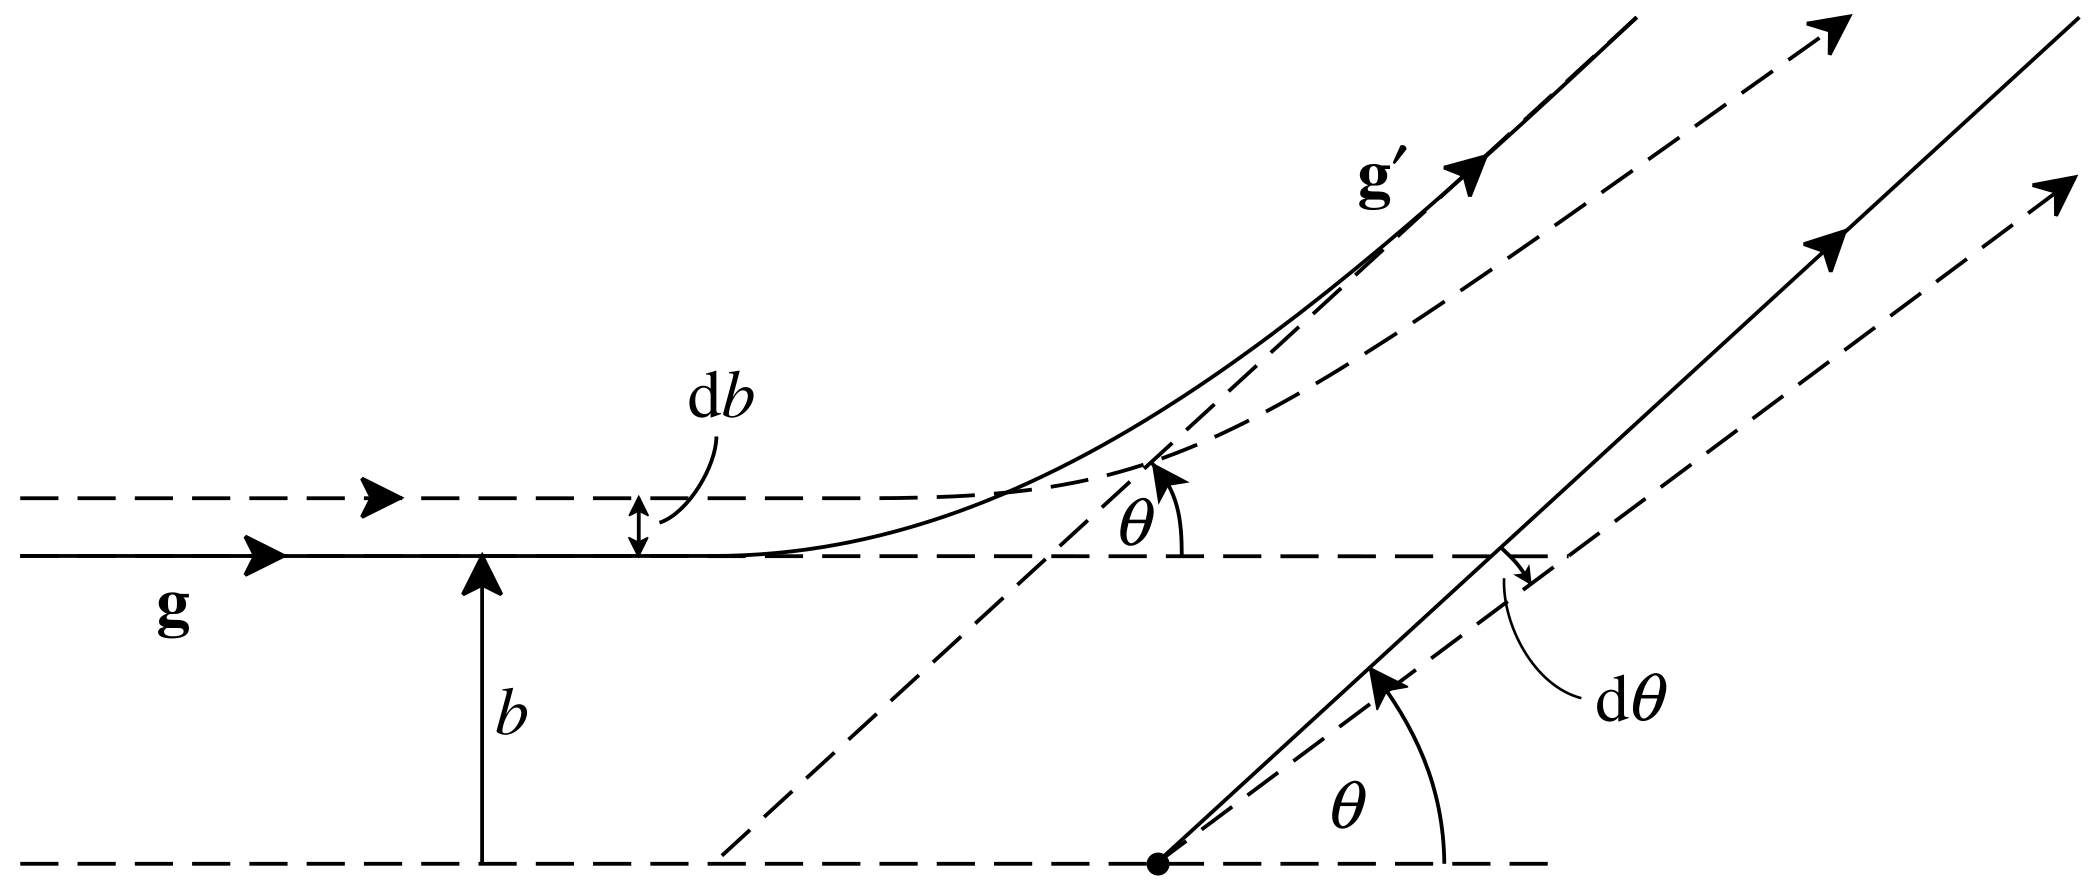
\includegraphics[width=0.60\textwidth]{figures/background/impact_parameter.png}
    \end{center}
    \caption{Scattering in the center of mass frame \cite{boyd_sanderson_2003_chapter84}.}
    \label{fig:scatteringCrossSection}
\end{figure}

The scattering angle is directly related to the impact parameter $b$ of the scatterer. As
aforementioned, the majority of collisions within the range of a Debye sphere are happening at large
impact parameters (i.e. small angles $\theta$).
With the Rutherford scattering cross-section,
$\sigma (\lvert \vect g \rvert, \theta) = - \frac{b}{\sin{\theta}} \frac{db}{d\theta}$,
one can then integrate over all possible scatterers of a certain velocity $\vect v_s$ and arrive at
the so called Rosenbluth potentials (simplified for single species plasma):

\begin{align}
    h(\vect v) &= 2 \int \frac{f(\vect v)}{\lVert \vect v - \vect v_s \rVert} d\vect v_s,
    \label{eq:rbFrictionIntegral} \eqVspace
    g(\vect v) &= \int \lVert \vect v - \vect v_s \rVert f(\vect v) d\vect v_s. \label{eq:rbDiffusionIntegral}
\end{align}

We can now succinctly write the two ensemble averages defined in Equation \ref{eq:fokkerPlanckTerm}
as

\begin{align}
    \vect F_d(\vect v) = \frac{\langle \Delta \vect v \rangle}{\Delta t} &= \Gamma \frac{\partial h(\vect
    v)}{\partial \vect v}, \label{eq:frictionCoeff} \eqVspace
    \matr D(\vect v) = \frac{\langle \Delta \vect v \Delta \vect v \rangle}{\Delta t} &= \Gamma
    \frac{\partial^2 g(\vect v)}{\partial \vect v \partial \vect v}, \label{eq:diffusionCoeff} 
\end{align}

with the common prefactor $\Gamma = \frac{q_e^4}{4\pi \epsilon_0^2 m_e^2} \ln{\Lambda}$ being a
function of the Coulomb logarithm $\ln \Lambda \approx 10$.
The term in Equation \ref{eq:frictionCoeff} is known as the \emph{dynamic friction} coefficient and Equation
\ref{eq:diffusionCoeff} as the \emph{dynamic diffusion} coefficient.

\section{Properties of Rosenbluth Potentials}
\label{section:rb_potentials}

It may not be obvious at first how to compute the integrals in Equations \ref{eq:rbFrictionIntegral} and
\ref{eq:rbDiffusionIntegral}. But we can find a strong similarity to potential theory (see
\cite{Callend2018Chapter223}) which allows us to reformulate them as

\begin{align}
    \velNabla^2 h(\vect v) &= -8 \pi f(\vect r, \vect v), \label{eq:rbFirstPotential} \eqVspace
    \velNabla^2 \velNabla^2 g(\vect v) &= -8 \pi f(\vect r, \vect v). \label{eq:rbSecondPotential}
\end{align}

As a result we can then directly employ well-established methods (as introduced in Chapter
\ref{chapter:computational_model}) for their computation.
Observing the matching right-hand side terms, it is easy to show that from Equations
\ref{eq:frictionCoeff} - \ref{eq:rbSecondPotential} we can establish following relations (cf.
\cite{FPOhakim})

\begin{equation}
    \begin{aligned}
        \text{Tr}(\matr D(\vect v)) &= \Gamma \velNabla^2 g(\vect v) \\
                                    &= \Gamma h(\vect v), \eqVspace
        \velNabla \cdot \matr D(\vect v) &= \velNabla \cdot (\Gamma \velNabla \velNabla g(\vect v)) \\
                                      &= \Gamma \velNabla \velNabla^2 g(\vect v) \\
                                      &= \vect F_d(\vect v) \\
                                      &= \Gamma \velNabla h(\vect v).
    \end{aligned}
    \label{eq:rb_identities}
\end{equation}

These yield an additional apparatus to further test whether an implementation is correct. We mention
this since one has to implement two different solvers to compute either potential and also, as we will
see, there exist multiple ways to numerically compute the \gls{fp} coefficients from the potentials.

The coefficients also possess some interesting properties as described in Hinton
\cite{hinton1983collisional} that will help us derive the numerical model explained in Chapter
\ref{chapter:computational_model}. The proofs of which are detailed therein, while we content 
ourselves by only summarizing the key points:

The distribution function cannot become negative ($f(\vect r, \vect v, t) \ge 0$) and as a
consequence the tensor $\partial^2 g(\vect v)/ \partial \vect v \partial \vect v$ is positive
semi-definite.
Therefore intuitively, one can think of the modeled Coulomb collisions ``filling" up any existing
areas close to zero in the phase space $f(\vect r, \vect v, t)$.


\section{Langevin Equation}
\label{section:langevin}

In the last section we touched upon the fact that the collision operator acts on a time-scale
where macroscopic properties of the phase space experience slow changes as a result of many random short
collisions.
These dynamics can also be characterized by the Langevin equation giving us a different view on the
problem, while also allowing us to integrate it with the \gls{pic} approach (see Section
\ref{section:PIC_method}).
Thus, it does not come as a surprise that we can show equivalence between the \gls{fp} and Langevin
description \cite{tabar2019}.
The Langevin equation describing the dynamics of $\vect v$ as a Markov process, takes on the
following form \cite{cadjan_ivanov_1999}:

\begin{equation}
    \vect v(t) = \vect F(\vect v) dt + \matr Q(\vect v)d\vect W(t),
    \label{eq:langevinEquation}
\end{equation}

where $\matr Q$ follows from the factorization of $\matr D = \matr Q^T \matr Q$ and $d\vect W(t)$ is
the randomly fluctuating Langevin force with zero mean and correlation function:

\begin{equation}
\label{eq:langevinForce}
\left\{  
\begin{aligned}
    \langle d \vect W_i(t) \rangle &= 0, \\
    \langle d \vect W_i(t) d \vect W_j(t') \rangle &= \delta_{ij} dt.
\end{aligned}
\right.
\end{equation}

As we will see in Section \ref{sub:stochastic_description} we can use this to define the time
evolution of the coupled Vlasov-Poisson-Fokker-Planck (\gls{vpfp}) equation.

\section{Disorder Induced Heating}
\label{section:dihProblem}

Ultracold plasma is governed by the very low kinetic energy of initially unstructured
(disordered) particles.
Due to inter-particle forces (i.e. Coulomb repulsion) they subsequently start to relax from an unstructured into a more
structured state with lower potential energy. This causes an increase in kinetic energy in form of
a heating process with increased particle velocities.
For simulating a plasma undergoing this process, the particle interactions can therefore not be regarded as a small
perturbation of the system dynamics anymore.

The \gls{dih} effect is known to limit the beam brightness of cold electron beams that emanate from
a photoemission source \cite{Maxson_2013}.
In the case of the Free Electron Laser Swiss\gls{fel} it has been observed by Prat et al.
\cite{prat2022energy} that their current simulation method cannot completely replicate the observed behavior
in the beamline.
One suspicion that has come up as an attempted explanation, is that the current method does not
capture the inter-particle collisions well.
Therefore we strive to implement a solver which enables to model these interactions in a more efficient manner than the
existing \gls{p3m} method by Ulmer \cite{p3m_ulmer}.

\subsubsection{Beam Emittance}

When simulating a particle bunch in an accelerator one needs a way to describe how it behaves over
time.
Beam emittance is a conserved quantity of motion that is based on the coordinates of the particles
in phase space.
Intuitively one can think of the emittance value as an area (by projection of the phase space) that
exhibits an ellipsoidal shape.

We can define the \gls{rms} emittance and normalized emittance along the first dimension by the central moments $\langle \cdot \rangle$ of the particle
distributions as follows:

\begin{align}
    \label{eq:rmsEmittance}
    \eps &= \sqrt{\bracket{\vect r_x^2} \bracket{\vect v_x^2} - \bracket{\vect r_x \vect
v_x}^2}, \\
\neps &= \sqrt{\bracket{\vect r_x^2} \bracket{(\gamma \beta_x)^2} - \bracket{\vect r_x \gamma
    \beta_x}^2} = \eps \gamma \beta_x,
\end{align}

where $\gamma = \left({1 - \left( \frac{v}{c} \right)^2} \right)^{-\frac{1}{2}}$ is the Lorentz factor and $\beta_x =
\frac{\vect v_x}{c}$ is the normalized transverse velocity.
As a bunch accelerates, the transverse size shrinks. Though, if we scale the \gls{rms} emittance by ($\gamma
\beta_x$), we can recover the invariant property of the emittance \cite{emittanceFloettmann}, hence
the formulation of normalized emittance $\neps$.

We will use the normalized emittance in order to validate the correctness of our simulation in
the \gls{dih} case (see Chapter \ref{chapter:results}).

\subsubsection{Plasma Frequency}

Cold plasma exhibits an oscillating behavior at a certain plasma frequency $\omega_p$.
It is a function of the number density $n_0$, the elementary charge $e$,
the electron mass $m_e$ and the vacuum permittivity $\varepsilon_0$:

\begin{equation}
    \omega_p = \sqrt{\frac{n_0 e^2}{m_e \varepsilon_0}}.
    \label{eq:plasmaFrequency}
\end{equation}

Following this definition we can define the plasma period as $\tau_p = 2\pi / \omega_p$.

% Plasmas in the ultracold regime are challenging to describe theoretically because they are strongly interacting, which means that interactions cannot be treated as a small perturbation.

